\documentclass{standalone}
\usepackage{tikz}
\usetikzlibrary{patterns, positioning}

\begin{document}
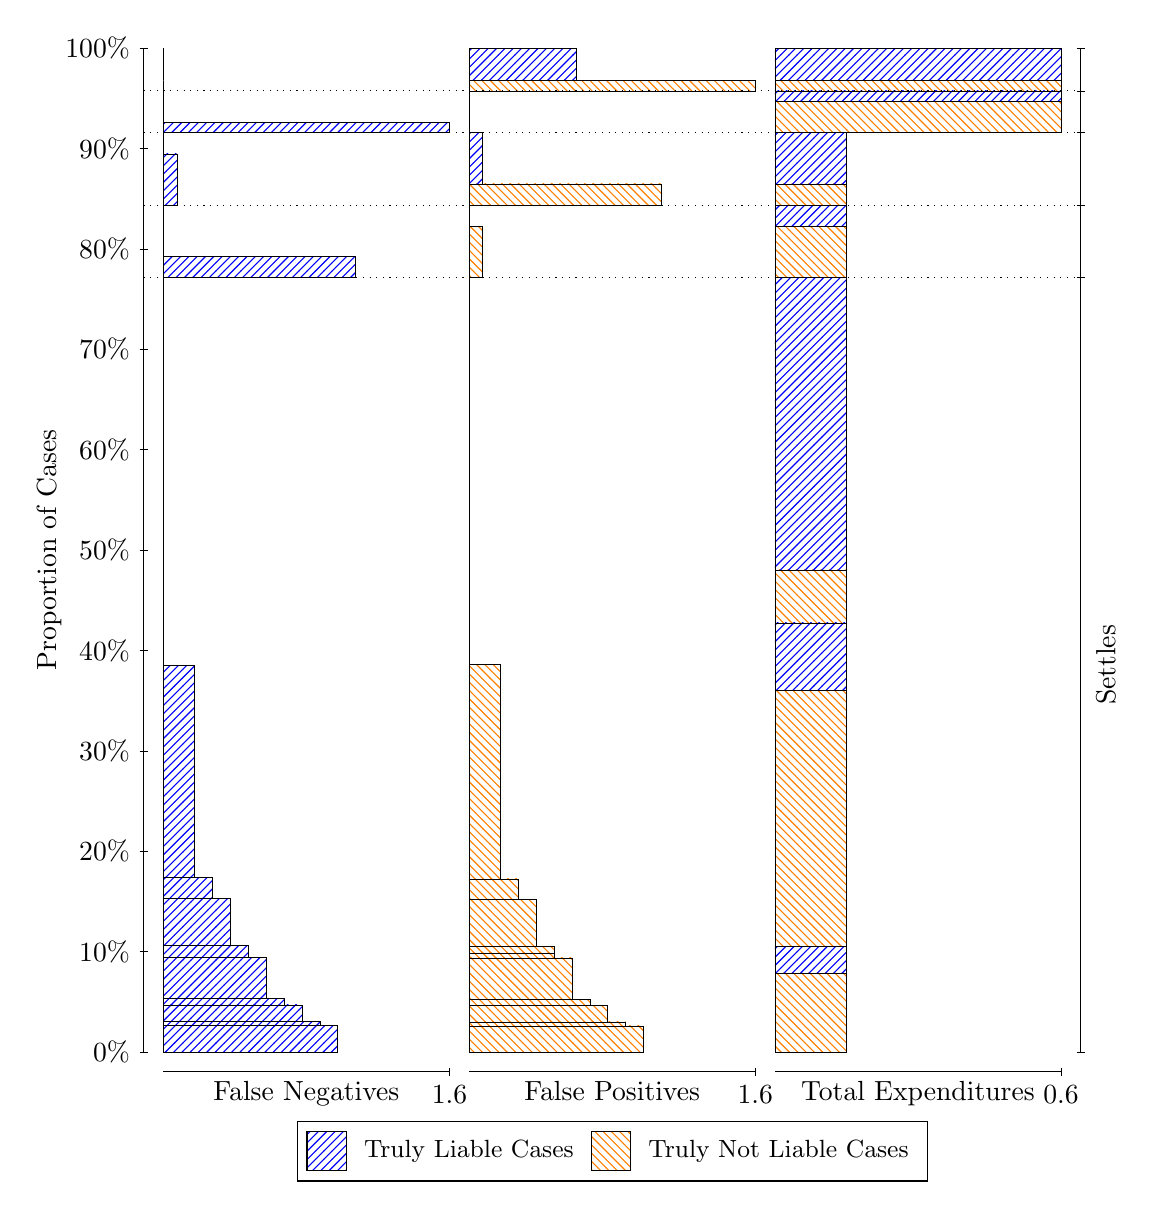
\begin{tikzpicture}
\draw[black, very thin] (1.5,1.75) -- (1.5,14.5);
\node[rotate=90, anchor=center] at (0.3, 8.125) {Proportion of Cases};
\draw[black, very thin] (1.45,1.75) -- (1.55,1.75);
\node[anchor=east] at (1.45, 1.75) {0\%};
\draw[black, very thin] (1.45,3.025) -- (1.55,3.025);
\node[anchor=east] at (1.45, 3.025) {10\%};
\draw[black, very thin] (1.45,4.3) -- (1.55,4.3);
\node[anchor=east] at (1.45, 4.3) {20\%};
\draw[black, very thin] (1.45,5.575) -- (1.55,5.575);
\node[anchor=east] at (1.45, 5.575) {30\%};
\draw[black, very thin] (1.45,6.85) -- (1.55,6.85);
\node[anchor=east] at (1.45, 6.85) {40\%};
\draw[black, very thin] (1.45,8.125) -- (1.55,8.125);
\node[anchor=east] at (1.45, 8.125) {50\%};
\draw[black, very thin] (1.45,9.4) -- (1.55,9.4);
\node[anchor=east] at (1.45, 9.4) {60\%};
\draw[black, very thin] (1.45,10.675) -- (1.55,10.675);
\node[anchor=east] at (1.45, 10.675) {70\%};
\draw[black, very thin] (1.45,11.95) -- (1.55,11.95);
\node[anchor=east] at (1.45, 11.95) {80\%};
\draw[black, very thin] (1.45,13.225) -- (1.55,13.225);
\node[anchor=east] at (1.45, 13.225) {90\%};
\draw[black, very thin] (1.45,14.5) -- (1.55,14.5);
\node[anchor=east] at (1.45, 14.5) {100\%};

\draw[black, very thin] (13.4,1.75) -- (13.4,14.5);
\draw[black, very thin] (13.35,1.75) -- (13.45,1.75);
\node[anchor=west] at (13.35, 1.75) {};
\draw[black, very thin] (13.35,11.583) -- (13.45,11.583);
\node[anchor=west] at (13.35, 11.583) {};
\draw[black, very thin] (13.35,12.505) -- (13.45,12.505);
\node[anchor=west] at (13.35, 12.505) {};
\draw[black, very thin] (13.35,13.426) -- (13.45,13.426);
\node[anchor=west] at (13.35, 13.426) {};
\draw[black, very thin] (13.35,13.955) -- (13.45,13.955);
\node[anchor=west] at (13.35, 13.955) {};
\draw[black, very thin] (13.35,14.5) -- (13.45,14.5);
\node[anchor=west] at (13.35, 14.5) {};

\draw[black, very thin, pattern color=blue, pattern=north east lines] (1.75,1.75) rectangle (3.9641,2.0871);
\draw[black, very thin, pattern color=blue, pattern=north east lines] (1.75,2.0871) rectangle (3.737,2.136);
\draw[black, very thin, pattern color=blue, pattern=north east lines] (1.75,2.136) rectangle (3.5099,2.3476);
\draw[black, very thin, pattern color=blue, pattern=north east lines] (1.75,2.3476) rectangle (3.2828,2.4259);
\draw[black, very thin, pattern color=blue, pattern=north east lines] (1.75,2.4259) rectangle (3.0557,2.9484);
\draw[black, very thin, pattern color=blue, pattern=north east lines] (1.75,2.9484) rectangle (2.8286,3.1032);
\draw[black, very thin, pattern color=blue, pattern=north east lines] (1.75,3.1032) rectangle (2.6016,3.6971);
\draw[black, very thin, pattern color=blue, pattern=north east lines] (1.75,3.6971) rectangle (2.3745,3.9719);
\draw[black, very thin, pattern color=blue, pattern=north east lines] (1.75,3.9719) rectangle (2.1474,6.6591);
\draw[black, very thin, pattern color=orange, pattern=north west lines] (1.75,6.6591) rectangle (1.75,11.583);
\draw[black, very thin, pattern color=blue, pattern=north east lines] (1.75,11.583) rectangle (4.1911,11.852);
\draw[black, very thin, pattern color=orange, pattern=north west lines] (1.75,11.852) rectangle (1.75,12.505);
\draw[black, very thin, pattern color=blue, pattern=north east lines] (1.75,12.505) rectangle (1.9203,13.157);
\draw[black, very thin, pattern color=orange, pattern=north west lines] (1.75,13.157) rectangle (1.75,13.426);
\draw[black, very thin, pattern color=blue, pattern=north east lines] (1.75,13.426) rectangle (5.3833,13.557);
\draw[black, very thin, pattern color=orange, pattern=north west lines] (1.75,13.557) rectangle (1.75,13.955);
\draw[black, very thin, pattern color=orange, pattern=north west lines] (1.75,13.955) rectangle (1.75,14.086);
\draw[black, very thin, pattern color=blue, pattern=north east lines] (1.75,14.086) rectangle (1.75,14.5);
\draw[black, very thin, pattern color=orange, pattern=north west lines] (5.6333,1.75) rectangle (7.8474,2.0827);
\draw[black, very thin, pattern color=orange, pattern=north west lines] (5.6333,2.0827) rectangle (7.6203,2.1324);
\draw[black, very thin, pattern color=orange, pattern=north west lines] (5.6333,2.1324) rectangle (7.3932,2.3446);
\draw[black, very thin, pattern color=orange, pattern=north west lines] (5.6333,2.3446) rectangle (7.1661,2.4222);
\draw[black, very thin, pattern color=orange, pattern=north west lines] (5.6333,2.4222) rectangle (6.9391,2.9439);
\draw[black, very thin, pattern color=orange, pattern=north west lines] (5.6333,2.9439) rectangle (6.712,3.0075);
\draw[black, very thin, pattern color=orange, pattern=north west lines] (5.6333,3.0075) rectangle (6.712,3.0954);
\draw[black, very thin, pattern color=orange, pattern=north west lines] (5.6333,3.0954) rectangle (6.4849,3.6844);
\draw[black, very thin, pattern color=orange, pattern=north west lines] (5.6333,3.6844) rectangle (6.2578,3.9492);
\draw[black, very thin, pattern color=orange, pattern=north west lines] (5.6333,3.9492) rectangle (6.0307,6.6737);
\draw[black, very thin, pattern color=blue, pattern=north east lines] (5.6333,6.6737) rectangle (5.6333,11.583);
\draw[black, very thin, pattern color=orange, pattern=north west lines] (5.6333,11.583) rectangle (5.8036,12.236);
\draw[black, very thin, pattern color=blue, pattern=north east lines] (5.6333,12.236) rectangle (5.6333,12.505);
\draw[black, very thin, pattern color=orange, pattern=north west lines] (5.6333,12.505) rectangle (8.0745,12.775);
\draw[black, very thin, pattern color=blue, pattern=north east lines] (5.6333,12.775) rectangle (5.8036,13.426);
\draw[black, very thin, pattern color=orange, pattern=north west lines] (5.6333,13.426) rectangle (5.6333,13.825);
\draw[black, very thin, pattern color=blue, pattern=north east lines] (5.6333,13.825) rectangle (5.6333,13.955);
\draw[black, very thin, pattern color=orange, pattern=north west lines] (5.6333,13.955) rectangle (9.2667,14.086);
\draw[black, very thin, pattern color=blue, pattern=north east lines] (5.6333,14.086) rectangle (6.9958,14.5);
\draw[black, very thin, pattern color=orange, pattern=north west lines] (9.5167,1.75) rectangle (10.425,2.7552);
\draw[black, very thin, pattern color=blue, pattern=north east lines] (9.5167,2.7552) rectangle (10.425,3.0941);
\draw[black, very thin, pattern color=orange, pattern=north west lines] (9.5167,3.0941) rectangle (10.425,6.3403);
\draw[black, very thin, pattern color=blue, pattern=north east lines] (9.5167,6.3403) rectangle (10.425,7.1999);
\draw[black, very thin, pattern color=orange, pattern=north west lines] (9.5167,7.1999) rectangle (10.425,7.8721);
\draw[black, very thin, pattern color=blue, pattern=north east lines] (9.5167,7.8721) rectangle (10.425,11.583);
\draw[black, very thin, pattern color=orange, pattern=north west lines] (9.5167,11.583) rectangle (10.425,12.236);
\draw[black, very thin, pattern color=blue, pattern=north east lines] (9.5167,12.236) rectangle (10.425,12.505);
\draw[black, very thin, pattern color=orange, pattern=north west lines] (9.5167,12.505) rectangle (10.425,12.775);
\draw[black, very thin, pattern color=blue, pattern=north east lines] (9.5167,12.775) rectangle (10.425,13.426);
\draw[black, very thin, pattern color=orange, pattern=north west lines] (9.5167,13.426) rectangle (13.15,13.825);
\draw[black, very thin, pattern color=blue, pattern=north east lines] (9.5167,13.825) rectangle (13.15,13.955);
\draw[black, very thin, pattern color=orange, pattern=north west lines] (9.5167,13.955) rectangle (13.15,14.086);
\draw[black, very thin, pattern color=blue, pattern=north east lines] (9.5167,14.086) rectangle (13.15,14.5);
\draw[black, dotted] (1.5,11.583) -- (13.4,11.583);
\draw[black, dotted] (1.5,12.505) -- (13.4,12.505);
\draw[black, dotted] (1.5,13.426) -- (13.4,13.426);
\draw[black, dotted] (1.5,13.955) -- (13.4,13.955);
\draw[black, very thin] (1.75,1.5) -- (5.3833,1.5);
\node[anchor=north] at (3.5667, 1.5) {False Negatives};
\draw[black, very thin] (5.3833,1.45) -- (5.3833,1.55);
\node[anchor=north] at (5.3833, 1.45) {1.6};

\draw[black, very thin] (5.6333,1.5) -- (9.2667,1.5);
\node[anchor=north] at (7.45, 1.5) {False Positives};
\draw[black, very thin] (9.2667,1.45) -- (9.2667,1.55);
\node[anchor=north] at (9.2667, 1.45) {1.6};

\draw[black, very thin] (9.5167,1.5) -- (13.15,1.5);
\node[anchor=north] at (11.333, 1.5) {Total Expenditures};
\draw[black, very thin] (13.15,1.45) -- (13.15,1.55);
\node[anchor=north] at (13.15, 1.45) {0.6};

\node[black, centered, rotate=90] at (13.72, 6.6664) {Settles};





\draw (7.449999999999999,1.5) node[draw=none] (baseCoordinate) {};
\begin{scope}[align=center]
        \matrix[scale=0.5, draw=black, below=0.5cm of baseCoordinate, nodes={draw}, column sep=0.1cm]{
            \node[rectangle, draw, minimum width=0.5cm, minimum height=0.5cm, pattern=north east lines, pattern color=blue] {}; &
            \node[draw=none, font=\small] (B) {Truly Liable Cases}; &
            \node[rectangle, draw, minimum width=0.5cm, minimum height=0.5cm, pattern=north west lines, pattern color=orange] {}; &
            \node[draw=none, font=\small] (B) {Truly Not Liable Cases}; \\
            };
\end{scope}

\end{tikzpicture}
\end{document}